\documentclass{article}
\usepackage[textwidth=5.5in,textheight=9in]{geometry}
\usepackage{amsmath,booktabs,hyperref,graphicx}
\makeatletter
\def\input@path{{../paper/}}
\makeatother
\title{Experiments and independent-model replication}
\author{}
\date{September 17, 2026}
\begin{document}
\maketitle
\noindent This preview preserves the original pilot results and appends the
completed independent-model check. The original HalfCheetah result concerns
one trained policy; the new subsection reports all eight fresh models and
the preregistered useful-effect decision. Neither section resolves the
theoretical proof TODOs in the supplied manuscript. A final retrospective
subsection examines error in the supplied safe set and adds conservative
projection and conditioning controls.
\input{../paper/pilot_experiments.tex}
\subsection{Independent-model replication}
We froze the previously promising HalfCheetah RMS-0.72 setting and trained eight new models with independent initialization and optimization seeds. The demonstration dataset and episode split were held fixed. Every model was evaluated at the same 64 fresh states with four replicates per state, without retuning or excluding weak models.

Refinement minus repaired BayesFP averaged 16.88 native-return points (95\% crossed model/state bootstrap interval [6.06, 28.29]; model-level t interval [8.83, 24.94]). The mean favored refinement in 7 of eight models. The preregistered useful-advantage criterion was NOT met. The threshold remained 26.19 points.

Conditioning minus projection was +0.98 [-2.70, +4.88]; refinement minus projection was +17.12 [+6.19, +28.18] (secondary descriptive 95\% intervals). These comparisons separate target utility from finite-sampler performance.

There were 0 rejection refusals and 0 hard-output violations. Raw BayesFP violated the initial-chunk constraint in 320/2048 outputs; its repaired arm had zero violations. The study remains conditional on one fixed demonstration dataset and does not establish general posterior accuracy or robust closed-loop diffusion locomotion.

\begin{figure}[t]
\centering
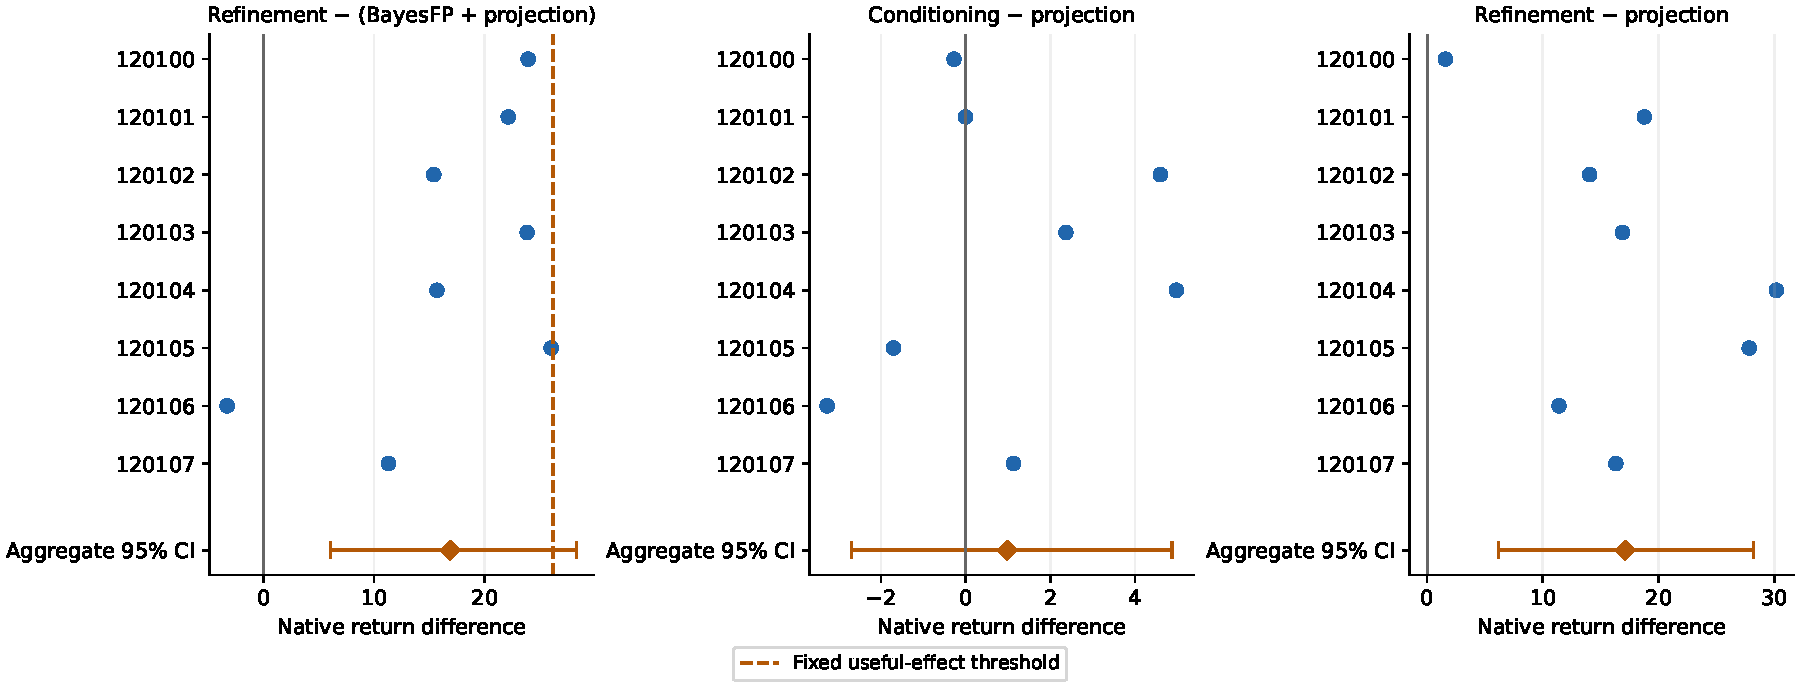
\includegraphics[width=\linewidth]{../../results/halfcheetah_replication/model_comparison.pdf}
\caption{Every independently trained model and the aggregate return differences.
The aggregate interval uses a crossed model/state bootstrap. The dashed line
marks the fixed 26.19-point useful-effect threshold for the primary comparison.
Secondary contrasts are descriptive. All models use the same fixed demonstration
dataset and the same fresh evaluation states.}
\end{figure}
\paragraph{Exploratory sensitivity to safe-set error.}
Using all eight frozen HalfCheetah policies, we re-evaluated each of the 2,048
outputs per arm against nearby effort caps, without changing its trajectory
or reward. This is a retrospective uniform-bias probe, not an evaluation of a
learned estimator. With a true cap 0.1\% below the supplied cap, exact global
projection violated the true cap in 17.53\% of outputs, exact conditioning in
0.88\%, finite refinement in 6.79\%, and repaired BayesFP in 16.11\%.
At 1\% error these rates were 22.75\%, 8.20\%, 24.46\%, and 21.04\%, respectively.
The conditioning--projection difference at 1\% was $-14.55$ percentage points
(exploratory 95\% crossed model/state bootstrap interval $[-17.77,-11.52]$);
the refinement--projection difference was $+1.71$ points ($[-3.37,6.79]$).
Thus finite refinement did not consistently inherit the reference's robustness.

As an uncertainty-aware control, we executed another 4,096 trajectories using
projection and conditioning on a fixed 1\%-smaller set. At 1\% bias this is the
true set, and its projection is the exact oracle projection. Both controls had
zero violations and zero rejection-budget failures. The margin changed projection
return by $+1.33$ points ($[-1.50,4.25]$), and conditioning on the same smaller set
differed from projection by $+0.43$ ($[-4.34,5.26]$). This control requires a valid
error bound supplied equally to both methods. It prevents attributing a benefit
to conditioning that conservative projection can obtain without detectable
task-quality loss. The outcomes are normalized effort-envelope violations,
not collisions: at 1\% bias the largest excess for the original hard-filtered
arms was at most 0.007201, with numerical tolerance $10^{-6}$.
These findings motivate testing geometric or dynamical estimator errors and
calibrated-margin baselines; they do not identify the dominant cause of harm
in general robotics tasks.

\begin{figure}[t]
\centering
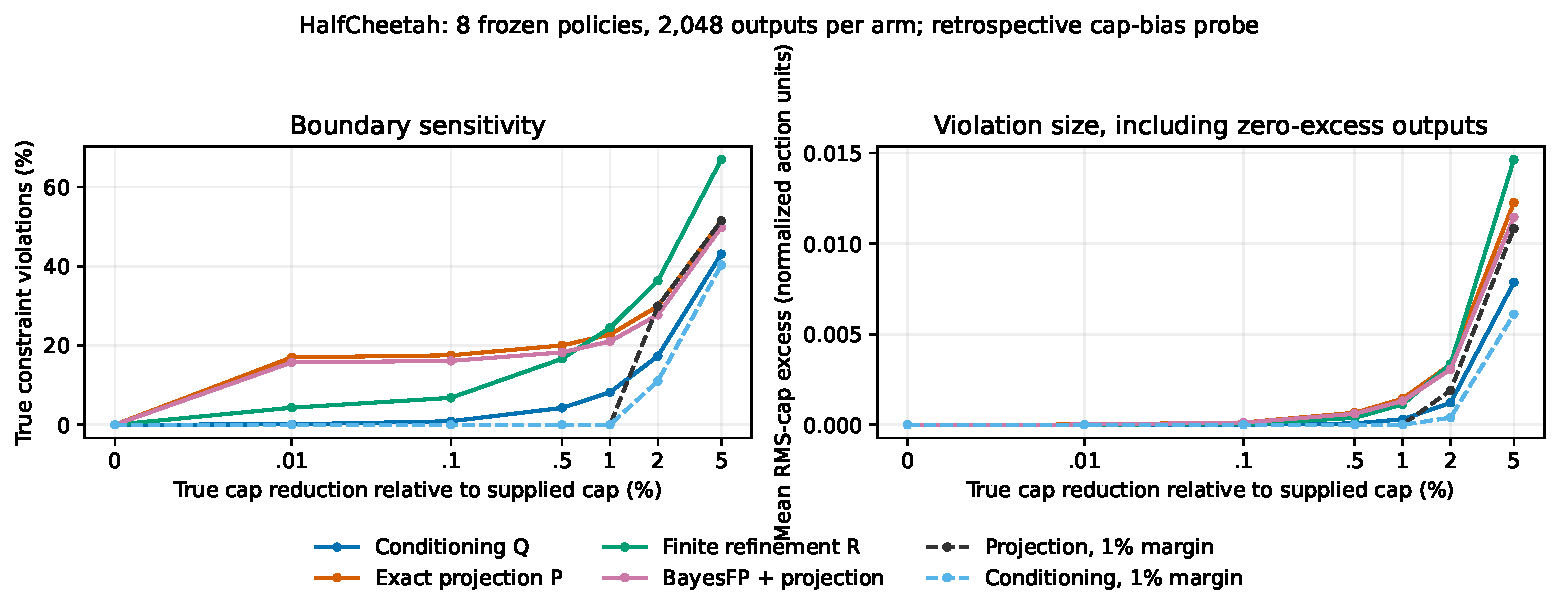
\includegraphics[width=\linewidth]{../../results/safe_set_mismatch/boundary_sensitivity.pdf}
\caption{Retrospective safe-set error probe. Each original arm reuses all
2,048 outputs from the eight-model study. The horizontal axis is linear near
zero and logarithmic beyond .01\% to display small errors. A valid 1\% margin
eliminates violations up to that bias, while finite refinement does not
uniformly inherit the conditional reference's boundary robustness. Violation
frequency and size are distinct; these are command-budget excesses, not
observed collisions. Lines connect the fixed evaluation grid.}
\end{figure}
\end{document}
